\documentclass{article}
\usepackage{amssymb}
\usepackage{ifsym}
\usepackage{pdfpages}
\begin{document}
	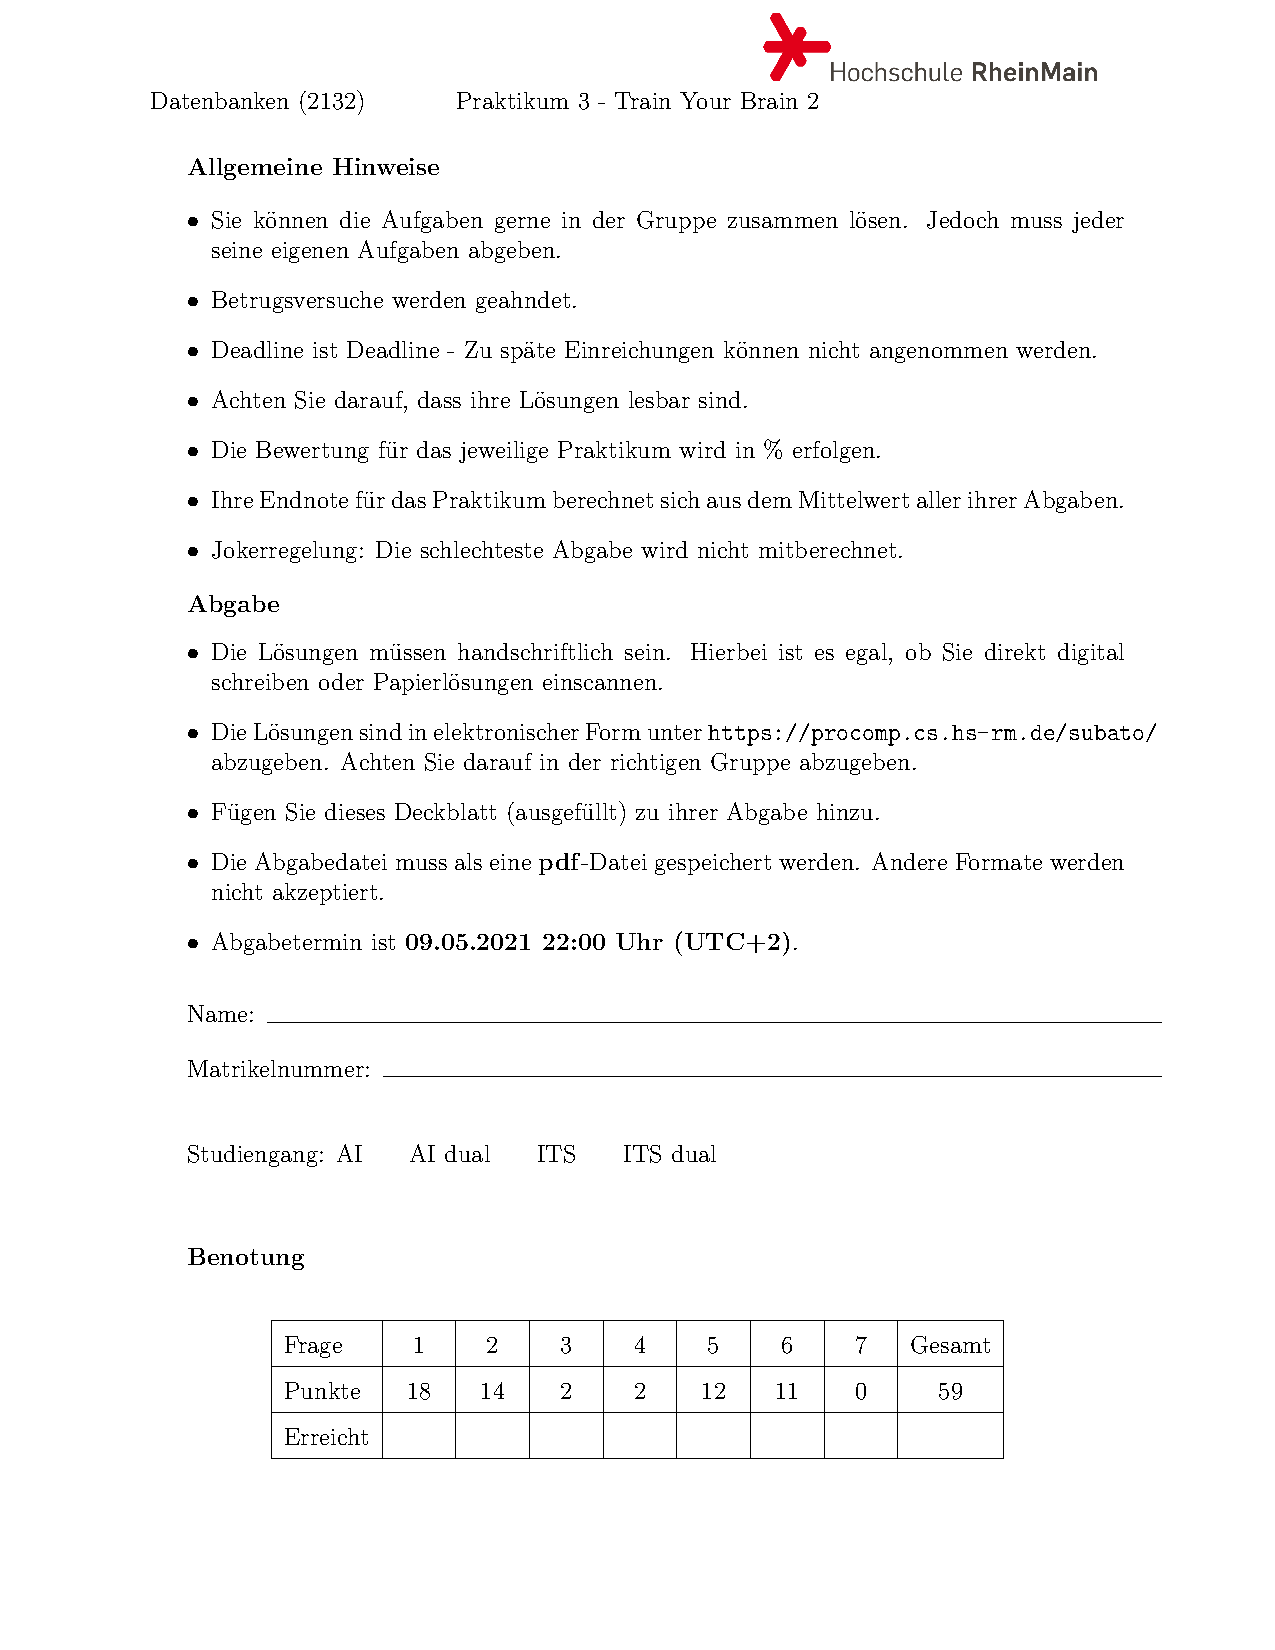
\includepdf[pages=1]{PA3_v2}
	\section*{Lsg Vorschlag DB Ü03 Maximilian Maag}
	Die Inhalted des PDF-Formulars sind leider beim Import in die Lösung verloren gegangen.. \\
	Maximilian Maag, Matnr: 1246281, AIdual
	\subsection*{Aufgabe 1}
	\subsection*{a)}
	R = 
	\begin{tabular}{c|c|c}
		a & b & c \\
		\hline
		\hline
		3 & 5 & 7 \\
		\hline
		3 & 5 & 7
	\end{tabular}
	\subsection*{b)}
	Der Inhalt der Frage ist nicht bestimmbar, da die Relation R kein Attribut 'd' besitzt.
	\subsection*{c)}
	R = 
	\begin{tabular}{c|c|c}
		a & b & c \\
		\hline
		\hline
		1 & 2 & 3
	\end{tabular}
	\subsection*{d)}
	R = \{\}
	\subsection*{e)}
	\begin{tabular}{c|c|c}
		a & b & c \\
		\hline
		\hline
		1 & 2 & 3 \\
		\hline
		3 & 5 & 7
	\end{tabular}
	\subsection*{f)}
	$\pi_{a \to b}(S) =$
	\begin{tabular}{c}
		a \\
		\hline
		8 \\
		5 \\
		1 \\
	\end{tabular}
	$\pi_{a}(R) = $
	\begin{tabular}{c}
		a \\
		\hline
		1 \\
		3 \\
		3 \\
	\end{tabular} \\
	$\delta(S.a \cup R.a)$ = 
	\begin{tabular}{c}
		a \\
		\hline
		8 \\
		5 \\
		1 \\
		3
	\end{tabular}
	\subsection*{g)}
	\begin{tabular}{c|c|c|c|c|c}
		R.a & R.b & R.c & S.b & S.c & S.d \\
		\hline
		\hline
		1 & 2 & 3 & 8 & 8 & 9 \\
		\hline
		1 & 2 & 3 & 5 & 7 & 9 \\
		\hline
		1 & 2 & 3 & 1 & 2 & 3 \\
		\hline
		3 & 5 & 7 & 8 & 8 & 9 \\
		\hline
		3 & 5 & 7 & 5 & 7 & 9 \\
		\hline
		3 & 5 & 7 & 1 & 2 & 3 \\
		\hline
		3 & 5 & 7 & 8 & 8 & 9 \\
		\hline
		3 & 5 & 7 & 5 & 7 & 9 \\
		\hline
		3 & 5 & 7 & 1 & 2 & 3 \\
	\end{tabular}
	\subsection*{h)}
	E = 
	\begin{tabular}{c|c|c|c|}
		R.a & R.b & R.c &  S.d \\
		\hline
		\hline
		3 & 5 & 7 & 9
	\end{tabular}
	\subsection*{i)}
	E = 
	\begin{tabular}{c|c|c|c|c}
		R.a & R.b & R.c & S.b & S.d \\
		\hline \hline
		1 & 2 & 3 & 1 & 3
	\end{tabular}
	\section*{Aufgabe 2}
	\subsection*{a)}
	max(m) = m \\
	min(m)  = 0
	\subsection*{b)}
	min = 1 \\
	max = m
	\subsection*{c)}
	max = m, min = m
	\subsection*{d)}
	max = m, min = m
	\subsection*{e)}
	min(m,n) = 1 \\
	max(m,n) = $m^{n}$
	\subsection*{f)}
	min(m,n) = 0 \\
	max(m,n) = m+n
	\subsection*{g)}
	min(m,n) = 0 \\
	max(m,n) = R * c S
	\section*{Aufgabe 3}
	$\delta_C$(R x S)
	\section*{Aufgabe 4}
	$\rho_{b}(\pi_{a}(S))$
	\section*{Aufgabe 5}
	\subsection*{a)}
	$\pi_{did}(\sigma_{gs=femal}(Drachen))$
	\subsection*{b)}
	$\pi_{did,name}(\sigma_{gj>1900}(Drachen))$
	\subsection*{c)}
	$\pi_{did}(\sigma_{Mutter>=20 ORE Mutter<=30 ORE Mutter>=20 ORE Mutter<=30}(Drachen))$
	\subsection*{d)}
	$\not\pi_{did}(\sigma_{Mutter>=20 ORE Mutter<=30 ORE Mutter>=20 ORE Mutter<=30}(Drachen))$
	\subsection*{e)}
	$\sigma_{name=Steffen ORE Art=3}(Drachen)$
	\section*{Aufgabe 6}
	\subsection*{a)}
	E =
	\begin{tabular}{c}
		namen \\
		\hline
		\hline
		Anna \\
		Steffen \\
		Markus \\
		Max
	\end{tabular}
	\subsection*{b)}
	E = 
	\begin{tabular}{c}
		Mutter \\
		\hline
		26 \\
		8 \\
		7  \\
		24 \\
		29 \\
		14 \\
		21 \\
		19 \\
		30
	\end{tabular}
 	\subsection*{c)}
 	E = 
 	\begin{tabular}{c}
 		Vater \\
 		\hline
 		\hline
 		10  \\
 		5 \\
 		14 \\
 		4 \\
 		18 \\
 		14 \\
 		26 \\
 		30 \\
 		12 \\
 		29 \\
 		11
 	\end{tabular}
 \subsection*{d)}
 Dragon = 
 \begin{tabular}{c|c|c}
 	alpha & beta & gamma \\
 	\hline
 	\hline
 	Ines & 20 & 76 \\
 	\hline
 	Anja & 10 & 249 \\
 	\hline
 	Anna & 28 & 113 \\
 	\hline
 	Dennis & 8 & 90 \\
 	\hline
 	Steffen & 36 & 387 \\
 	\hline
 	Kevin & 28 & 376 \\
 	\hline
 	Steffen & 52 & 134 \\
 	\hline
 	Markus & 60 & 147 \\
 	\hline
 	Alexander & 24 & 221 \\ 
 	\hline
 	Max & 58 & 290 \\
 	\hline
 	Marco & 22 & 134 	
 \end{tabular}
\subsection*{e)}
Drachen1 = 
\begin{tabular}{c|c|c}
	name & mutter & vater \\
	\hline
	Ines & 26 & 10 \\
	\hline
	Anja & 14 & 5 \\
	\hline
	Anna & 8 & 14 \\
	\hline
	Dennis & 7 & 4 \\
	\hline
	Steffen & 24 & 18 \\
	\hline
	Kevin & 29 & 14 \\
	\hline
	Steffen & 14 & 26 \\
	\hline
	Markus & 19 & 30 \\
	\hline
	Alexander & 21 & 12 \\ 
	\hline
	Max & 19 & 29 \\
	\hline
	Marco & 30 & 11 
\end{tabular}
\subsection*{Aufgabe 7}
R $\cap$ S = $\pi_{alle Attribute von R}(R \bowtie S)$ \\
R - S = R $\ltimes$ S
\end{document}